\documentclass[12pt]{article}
\usepackage[utf8]{inputenc}
\usepackage{graphicx}
\usepackage{amsmath}
\usepackage{amsfonts}

\title{DD Lab 3 Assignment}
\author{Sai Kartik \\2020A3PS0435P}

\begin{document}
    \maketitle
    \section{Adder/Subtractor circuit}
        \subsection{Half adder circuit}
        \begin{center}
            \begin{figure}[ht]
                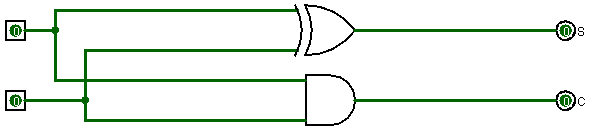
\includegraphics[scale=0.50]{halfadder.png}
            \end{figure}
        \end{center}
    \subsection{Full adder circuit}
    \begin{center}
        \begin{figure}[ht]
            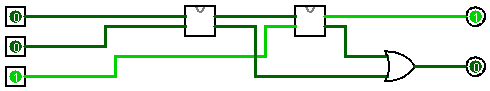
\includegraphics[scale=0.50]{fulladder.png}
            \caption{The boxes in this circuit are the half adders}
        \end{figure}
    \end{center}
    \newpage
    \subsection{4 bit adder}
    \begin{center}
        \begin{figure}[ht]
            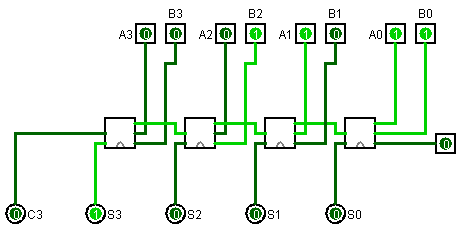
\includegraphics[scale=0.50]{4adder.png}
            \caption{The boxes in this circuit are the full adders}
        \end{figure}
    \end{center}
    \subsection{Adder/subtractor circuit}
    \begin{center}
        \begin{figure}[ht]
            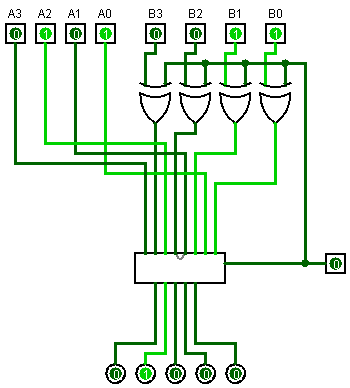
\includegraphics[scale=0.50]{addsub.png}
            \caption{The box in this circuit is the 4 bit adder}
        \end{figure}
    \end{center}
    \section{Subtractor circuits}
    \subsection{Half Subtractor}
    \begin{center}
        \begin{figure}[ht]
            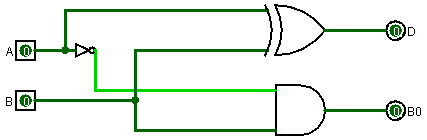
\includegraphics[scale=0.50]{halfsub.png}
        \end{figure}
    \end{center}
    \subsection{Full subtractor}
    \begin{center}
        \begin{figure}[ht]
            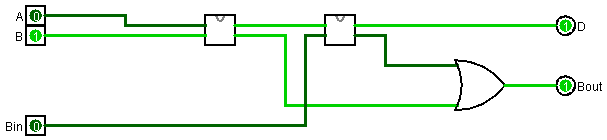
\includegraphics[scale=0.50]{fullsub.png}ca
            \caption{The box in the circuit is the half subtractor}
        \end{figure}
    \end{center}
\end{document}